\chapter{聚合物：合成、结构与性质}\label{ch:b2:polymer-synthesis}

尼龙长袜于 1939 年上市。它诞生于一个实验室，该实验室数年前着手研究
小分子如何连接成长分子，并在研究过程中得到一个让每位化学家初次接触时都会感到惊讶的结论：
对于由分子首尾相连而成的聚合物，99~\% 的产率是不够的。
本章解释其中的原因，描述链增长的两种方式，
并联系链的结构与材料的性质。
% ledger: hist:nylon-production-1939

\begin{recall}
第 1 册：聚合物、单体与重复单元、加成聚合物与缩聚物、热塑性塑料与热固性塑料。
本科一年级分册：自由基与均裂、碳正离子与
碳负离子、稳态近似。\Cref{ch:b2:acyl-substitution}：酯与酰胺。
\Cref{ch:b2:catalytic-cycles}：插入金属–碳键。
\end{recall}

\section{链及其摩尔质量}

\begin{definition}[聚合物]\label{def:b2:polymer-synthesis:polymer}
由大分子构成的物质称为\emph{聚合物}\index{聚合物}，每个大分子由小分子
重复连接而成，这些小分子即\emph{单体}\index{单体}。\emph{重复单元}\index{重复单元}
是其重复即构成链的最小原子团；链的\emph{聚合
度}\index{聚合度} $X$ 为链中所含单体来源单元的
数目。
\end{definition}

合成聚合物的样品从来不是由完全相同的链构成的，而是
由长度不同的链组成的混合物，其摩尔质量是一个平均值，平均方式取决于如何计数这些链。

\begin{definition}[摩尔质量的平均值]\label{def:b2:polymer-synthesis:averages}
对于含有 $N_i$ 条摩尔质量为 $M_i$ 的链的样品，其\emph{数均
摩尔质量}\index{数均摩尔质量}与\emph{重均摩尔质量}\index{重均摩尔质量}
分别为
\begin{equation*}
\bar M_n = \frac{\sum_i N_i M_i}{\sum_i N_i}, \qquad
\bar M_w = \frac{\sum_i N_i M_i^2}{\sum_i N_i M_i} = \sum_i w_i M_i,
\end{equation*}
其中 $w_i$ 为质量为 $M_i$ 的链的质量分数。\emph{分散度}\index{分散度}
$\text{\DH} = \bar M_w/\bar M_n$ 至少为 1，且仅当所有链的质量相同时
才等于 1。聚合度的平均值 $\bar X_n$ 与 $\bar X_w$
以相同的方式定义。
\end{definition}

数均对每条链计一次数；重均则按每条链的质量加权，因此
长链所占比重更大。$\text{\DH} \ge 1$ 即不等式 $\left(\sum N_i M_i\right)^2 \le
\sum N_i \sum N_i M_i^2$（柯西–施瓦茨不等式），等号仅当所有 $M_i$ 相等时成立。

\begin{method}[计算平均值]\label{met:b2:polymer-synthesis:averages}
\begin{enumerate}
  \item 将数据化为物质的量 $N_i$（或链的条数）与质量 $M_i$；由质量分数可得
        $N_i \propto w_i/M_i$。
  \item $\bar M_n = \sum N_i M_i / \sum N_i$；等价地，$1/\bar M_n = \sum w_i/M_i$。
  \item $\bar M_w = \sum w_i M_i$。
  \item $\text{\DH} = \bar M_w/\bar M_n$；检验 $\bar M_w \ge \bar M_n$。
\end{enumerate}
\end{method}

\section{逐步聚合与链式聚合}

\begin{definition}[逐步聚合与链式聚合]\label{def:b2:polymer-synthesis:step-chain}
在\emph{逐步聚合}\index{逐步聚合}中，任意两个带有互补官能团的分子
（单体、低聚物或长链）均可发生反应，链通过彼此连接而增长，
如聚酯、聚酰胺。在\emph{链式
聚合}\index{链式聚合}，一个活性中心（自由基、离子或金属–碳
键）每次将一个单体分子加到增长链的末端，如烯烃的聚合物。
\end{definition}

\begin{method}[逐步还是链式？]\label{met:b2:polymer-synthesis:classify}
\begin{enumerate}
  \item 单体带有两个能与对方基团反应的官能团（如酸与醇，
        酸与胺），常伴随放出小分子：逐步聚合。
  \item 单体含 \ce{C=C} 双键（或张力环）并带有引发剂：链式聚合。
  \item 由反应进程核对：在逐步聚合中，单体很早就消失，
        长链只在最后才出现；在链式聚合中，长链从一开始就出现，
        而单体逐渐被消耗。
\end{enumerate}
\end{method}

\subsection*{逐步聚合}

取 \ce{A-A} 与 \ce{B-B} 单体（二胺与二酸）的等比例混合物，或单一的
\ce{A-B} 单体。设 $p$ 为\emph{反应进度}：某一种官能团中已发生反应的
分数。

\begin{theorem}[卡罗瑟斯方程]\label{thm:b2:polymer-synthesis:carothers}
在恰好等比例的双官能单体的逐步聚合中，以单体单元计的数均
聚合度为
\begin{equation*}
\bar X_n = \frac{1}{1 - p}.
\end{equation*}
\end{theorem}

\begin{proof}
设起始有 $N_0$ 个单体分子，含 $N_0$ 个 \ce{A} 基团与 $N_0$ 个 \ce{B} 基团。每一次
\ce{A} 与 \ce{B} 之间的反应将两个分子连成一个，因此分子数减少
一个。发生 $pN_0$ 次反应后，剩余 $N = N_0 - pN_0 = N_0(1-p)$ 个分子，它们共享
$N_0$ 个单体单元：$\bar X_n = N_0/N = 1/(1-p)$。
\end{proof}

\begin{corollary}[不平衡]\label{cor:b2:polymer-synthesis:imbalance}
若官能团不平衡，设 $r = N_{\ce{A}}/N_{\ce{B}} \le 1$，且 $p$ 为
少数基团 \ce{A} 的反应进度，则
\begin{equation*}
\bar X_n = \frac{1 + r}{1 + r - 2rp}, \qquad \text{至多为 } \frac{1+r}{1-r} \text{ 当 } p = 1.
\end{equation*}
\end{corollary}

\begin{proof}
起始时有 $(N_{\ce{A}} + N_{\ce{B}})/2$ 个双官能单体分子。每个线型
分子有两个链端，每个链端各含一个未反应的基团；反应后剩余 $N_{\ce{A}}(1-p)$
个 \ce{A} 基团与 $N_{\ce{B}} - pN_{\ce{A}}$ 个 \ce{B} 基团，因此分子数为 $N = [N_{\ce{A}}(1-p) + N_{\ce{B}} -
pN_{\ce{A}}]/2$。相除，并以 $N_{\ce{B}} = N_{\ce{A}}/r$ 代入：
$\bar X_n = (1 + 1/r)/(1 - 2p + 1/r) = (1+r)/(1 + r - 2rp)$。取 $r = 1$ 即得卡罗瑟斯方程。
\end{proof}

方程解释了这一“钩子”现象。当 $p = 0.99$ 时，即连接反应的“99~\% 产率”，$\bar X_n =
100$；可用的纤维需要约此值或更高，因此连接反应必须超过 99~\%，并且单体须纯净
且严格等量配比，并不断移除反应放出的小分子（水、甲醇），以推动
平衡。即使转化完全，某一单体过量 1~\% 也会将 $\bar X_n$ 限制在 201。

\begin{theorem}[弗洛里分布]\label{thm:b2:polymer-synthesis:flory}
在反应进度为 $p$ 的逐步聚合中，若每个基团的反应活性
与其所在链的长度无关，则含 $x$ 个结构单元的链的数分数与质量分数分别为
\begin{equation*}
n_x = (1-p)\,p^{\,x-1}, \qquad w_x = x(1-p)^2 p^{\,x-1},
\end{equation*}
且 $\bar X_n = 1/(1-p)$，$\bar X_w = (1+p)/(1-p)$，故 $\text{\DH} = 1 + p$，在高
转化率时接近 2。
\end{theorem}

\begin{proof}
从链的一端追踪（为简便起见，取一个 \ce{A-B} 单体）。链上每个键以
概率 $p$ 独立形成。链恰含 $x$ 个单元，当且仅当前 $x-1$ 个键已形成，
而下一个键未形成，其概率为 $p^{\,x-1}(1-p)$，即 $n_x$。利用 $\sum_{x\ge1} p^{\,x-1} =
1/(1-p)$ 及其导数 $\sum x p^{\,x-1} = 1/(1-p)^2$ 与 $\sum x^2 p^{\,x-1} = (1+p)/(1-p)^3$：
得 $\sum n_x = 1$，$\bar X_n = \sum x n_x = 1/(1-p)$，$w_x = x n_x/\bar X_n = x(1-p)^2p^{\,x-1}$，且
$\bar X_w = \sum x w_x = (1-p)^2(1+p)/(1-p)^3 = (1+p)/(1-p)$。
\end{proof}

\begin{omfigure}
\begin{tikzpicture}
\begin{axis}[width=0.46\linewidth, height=5cm, xmin=0, xmax=400, ymin=0,
  xlabel={聚合度 $x$}, ylabel={质量分数 $w_x$}, label style={font=\small},
  tick label style={font=\scriptsize}, scaled y ticks=false,
  yticklabel style={/pgf/number format/fixed, /pgf/number format/precision=3},
  legend style={font=\scriptsize, at={(0.98,0.98)}, anchor=north east}, legend cell align=left]
\addplot[omDef, thick] table[x=x, y=p95] {figdata/out/bachelor-2-polymer-distributions-a.dat};
\addplot[omThm, thick] table[x=x, y=p98] {figdata/out/bachelor-2-polymer-distributions-a.dat};
\addplot[omMeth, thick] table[x=x, y=p99] {figdata/out/bachelor-2-polymer-distributions-a.dat};
\legend{$p = 0.95$, $p = 0.98$, $p = 0.99$}
\end{axis}
\end{tikzpicture}\hfill
\begin{tikzpicture}
\begin{axis}[width=0.46\linewidth, height=5cm, xmin=0, xmax=1, ymin=0, ymax=200,
  xlabel={反应进度 $p$}, ylabel={$\bar X_n$}, label style={font=\small},
  tick label style={font=\scriptsize}, xtick={0,0.2,0.4,0.6,0.8,1}]
\addplot[omDef, thick] table[x=p, y=Xn] {figdata/out/bachelor-2-polymer-distributions-b.dat};
\end{axis}
\end{tikzpicture}

{\small 逐步聚合（模型）。左：弗洛里质量分布
（见\cref{thm:b2:polymer-synthesis:flory}）；峰值位于 $\bar X_n$ 附近，且随其
向外移动而变宽。右：卡罗瑟斯方程；$\bar X_n$ 在 $p$ 非常接近 1 之前始终较小。}
% figdata: bachelor-2/polymer-distributions.py parts a, b
\end{omfigure}

\subsection*{自由基链增长}

\begin{definition}[链式聚合的步骤]\label{def:b2:polymer-synthesis:chain-steps}
自由基链式聚合分为三类步骤。在\emph{链引发}\index{链引发}中，一个
\emph{自由基引发剂}\index{自由基引发剂}（一种含弱键的分子，如过氧化物或
偶氮化合物）受热分解为自由基，其中一个自由基加成到单体上。在
\emph{链增长}\index{链增长}中，链端的自由基加成一个单体分子，并
仍为自由基。在\emph{链终止}\index{链终止}中，两个自由基相互销毁，方式为偶合
（二者成键）或歧化（其中一个自由基夺取另一个的氢原子）。
\end{definition}

\begin{omfigure}
\begin{align*}
&\text{链引发：} && \mathrm{I{-}I} \longrightarrow 2\,\mathrm{I^{\bullet}}, \qquad
\mathrm{I^{\bullet} + CH_2{=}CHPh \longrightarrow I{-}CH_2{-}\dot{C}HPh} \\
&\text{链增长：} && {\sim}\mathrm{CH_2{-}\dot{C}HPh + CH_2{=}CHPh \longrightarrow}\;
{\sim}\mathrm{CH_2{-}CHPh{-}CH_2{-}\dot{C}HPh} \\
&\text{链终止：} && {\sim}\mathrm{CH_2{-}\dot{C}HPh + Ph\dot{C}H{-}CH_2}{\sim} \longrightarrow
{\sim}\mathrm{CH_2{-}CHPh{-}CHPh{-}CH_2}{\sim}
\end{align*}

{\small 苯乙烯的自由基聚合。引发剂 \ce{I-I}（例如过氧化二苯甲酰）
分解为两个自由基；每个自由基加成到苯乙烯的 \ce{CH2} 端，生成更稳定的苄基
自由基；链增长使该加成重复数千次；两个链自由基偶合，使两条
链同时终止。点表示未成对电子。}
\end{omfigure}

\begin{theorem}[自由基聚合速率]\label{thm:b2:polymer-synthesis:radical-rate}
设引发剂的分解速率常数为 $k_d$，效率为 $f$（即引发链的
自由基所占比例），链增长速率常数为 $k_p$，链终止速率常数为 $k_t$（终止速率为 $2k_t
[\mathrm{M^\bullet}]^2$），则稳态下的聚合速率为
\begin{equation*}
R_p = k_p [\mathrm M] \sqrt{\frac{f k_d [\mathrm I]}{k_t}}.
\end{equation*}
\end{theorem}

\begin{proof}
设 $[\mathrm{M^\bullet}]$ 为所有链自由基的总浓度，不论其长度。它们
以速率 $R_i = 2fk_d[\mathrm I]$ 生成（每个引发剂分子产生两个自由基，其中比例为 $f$ 的
自由基引发链），并以速率 $2k_t[\mathrm{M^\bullet}]^2$ 消耗；链增长使一个链自由基
转化为另一个，不改变其数目。对
$[\mathrm{M^\bullet}]$ 应用稳态近似，得 $2fk_d[\mathrm I] = 2k_t[\mathrm{M^\bullet}]^2$，故 $[\mathrm{M^\bullet}] =
\sqrt{fk_d[\mathrm I]/k_t}$。单体主要通过链增长被消耗，速率为 $R_p =
k_p[\mathrm M][\mathrm{M^\bullet}]$。
\end{proof}

\begin{definition}[动力学链长]\label{def:b2:polymer-synthesis:chain-length}
\emph{动力学链长}\index{动力学链长} $\nu$ 是每个引发链的自由基平均加成的单体
分子数：$\nu = R_p/R_i$。
\end{definition}

\begin{proposition}[链长与引发剂]\label{prop:b2:polymer-synthesis:chain-length}
在稳态下，$\nu = k_p[\mathrm M]/\bigl(2\sqrt{fk_dk_t[\mathrm I]}\bigr)$：引发剂越多，
聚合越快，但链越短。若为偶合终止，则 $\bar X_n = 2\nu$；若为
歧化终止，则 $\bar X_n = \nu$。
\end{proposition}

\begin{proof}
$\nu = R_p/R_i = k_p[\mathrm M]\sqrt{fk_d[\mathrm I]/k_t}/(2fk_d[\mathrm I]) =
k_p[\mathrm M]/\bigl(2\sqrt{fk_dk_t[\mathrm I]}\bigr)$。每条开始的链平均加成 $\nu$ 个单体；
偶合使两条这样的链连成一个分子，歧化则留下两个分子。
\end{proof}

\begin{definition}[活性聚合]\label{def:b2:polymer-synthesis:living}
称\emph{活性聚合}\index{活性聚合}为不含链终止或链转移的链式聚合：
所有链同时开始，只要仍有单体便持续增长，
加入新单体后又恢复增长。苯乙烯在干燥的非质子性溶剂中以丁基锂引发
阴离子聚合，是典型例子。
\end{definition}

\begin{proposition}[窄分布]\label{prop:b2:polymer-synthesis:living}
在所有链同时开始的活性聚合中，聚合度服从
泊松分布，且 $\text{\DH} = 1 + \nu/(1+\nu)^2 \approx 1 + 1/\bar X_n$，其中 $\nu$ 为
每条链平均加入的单体数。
\end{proposition}

\admitted

该分布是同一时间内每条链所作加成次数的分布，这些加成是以相同速率发生的独立随机事件；
分散度由泊松分布的均值与方差导出，
二者均等于 $\nu$。由此，含 100 个链节的活性链 $\text{\DH} \approx 1.01$，
而同样平均长度的逐步聚合则接近 2。

\begin{omfigure}
\begin{tikzpicture}
\begin{axis}[width=0.72\linewidth, height=5cm, xmin=0, xmax=150, ymin=0,
  xlabel={聚合度 $x$}, ylabel={质量分数 $w_x$}, label style={font=\small},
  tick label style={font=\scriptsize}, scaled y ticks=false,
  yticklabel style={/pgf/number format/fixed, /pgf/number format/precision=3},
  legend style={font=\scriptsize, at={(0.98,0.98)}, anchor=north east}, legend cell align=left]
\addplot[omThm, thick] table[x=x, y=poisson] {figdata/out/bachelor-2-polymer-distributions-c.dat};
\addplot[omDef, thick] table[x=x, y=flory] {figdata/out/bachelor-2-polymer-distributions-c.dat};
\legend{活性（泊松）, 逐步聚合（弗洛里）}
\end{axis}
\end{tikzpicture}

{\small 两份样品的平均聚合度均为 $\bar X_n = 50$（模型）。活性链集中在 50 附近（$\text{\DH}
\approx 1.02$）；逐步聚合链则从单体一直分布到数百个链节（$\text{\DH} \approx
1.98$）。}
% figdata: bachelor-2/polymer-distributions.py part c
\end{omfigure}

\begin{definition}[共聚物]\label{def:b2:polymer-synthesis:copolymer}
由两种或两种以上不同单体构成的聚合物称为\emph{共聚物}\index{共聚物}，其链节
可无规排列（统计共聚物）、交替排列，或各自连成长段（嵌段
共聚物，由活性聚合制得），或以一种单体的链作为侧链接枝于另一种的主链上（接枝
共聚物）。
\end{definition}

\section{链的结构}

\begin{definition}[立构规整性]\label{def:b2:polymer-synthesis:tacticity}
在乙烯基聚合物 \ce{-[CH2-CHR]_n-} 中，每个 \ce{CHR} 碳都是手性碳原子。
\emph{立构规整性}\index{立构规整性}描述将主链画成平面锯齿形时它们的相对构型：
在\emph{全同立构}\index{全同立构}链中，所有 \ce{R} 基团位于平面的同一侧，
在\emph{间同立构}\index{间同立构}链中则交替排列，而在
\emph{无规立构}\index{无规立构}链中则随机排列。
\end{definition}

\begin{omfigure}
\setchemfig{atom sep=1.5em}
\begin{tabular}{rl}
\small 全同立构 & \chemfig{[:-30]-[:30](<[:90])-[:-30]-[:30](<[:90])-[:-30]-[:30](<[:90])-[:-30]-[:30](<[:90])-[:-30]-[:30](<[:90])-[:-30]} \\[2pt]
\small 间同立构 & \chemfig{[:-30]-[:30](<[:90])-[:-30]-[:30](<:[:90])-[:-30]-[:30](<[:90])-[:-30]-[:30](<:[:90])-[:-30]-[:30](<[:90])-[:-30]} \\[2pt]
\small 无规立构 & \chemfig{[:-30]-[:30](<[:90])-[:-30]-[:30](<[:90])-[:-30]-[:30](<:[:90])-[:-30]-[:30](<[:90])-[:-30]-[:30](<:[:90])-[:-30]}
\end{tabular}
\par\vspace{6pt}

{\small 聚丙烯画成纸面内的锯齿形，每个甲基为楔形（指向
读者）或虚楔形（背离读者）。全同立构：甲基均在同侧；间同立构：交替排列；
无规立构：杂乱无章。}
\end{omfigure}

规整的链能够并排堆积成结晶区，不规整的则不能。
全同立构聚丙烯由本科三年级分册中的金属催化剂制得，部分结晶，质硬、熔点高；
无规立构聚丙烯则是柔软、发黏的非晶态材料。聚合物很少完全结晶，
微晶嵌于链相互缠结的非晶区中。

\begin{definition}[热转变]\label{def:b2:polymer-synthesis:transitions}
聚合物的\emph{结晶度}\index{结晶度}是指其位于结晶区的
质量分数。\emph{玻璃化转变温度}\index{玻璃化转变温度}
$T_g$ 是这样一个温度：低于它时，非晶区为刚性玻璃，链段无法运动；
高于它时则变为橡胶态；结晶区则在更高的温度
$T_m$ 时熔化。
\end{definition}

聚苯乙烯与聚甲基丙烯酸甲酯均为非晶态，$T_g$ 高于室温：刚性的
透明玻璃。天然橡胶的 $T_g$ 远低于室温。聚乙烯的 $T_g$ 远低于
室温，但结晶度很高，坚韧而柔软：其微晶把处于橡胶态的
非晶部分维系在一起。

\begin{omfigure}
\begin{tikzpicture}[x=1cm, y=1cm]
\draw[->] (0,0) -- (8.6,0) node[below left, font=\small] {温度};
\draw[->] (0,0) -- (0,4.6) node[above, font=\small] {$\log$ 模量};
\draw[omDef, very thick] (0.2,4) .. controls (1.8,3.95) and (2.4,3.9) .. (2.8,3.6)
  .. controls (3.3,3.0) and (3.4,1.9) .. (4.0,1.75) -- (6.0,1.6)
  .. controls (6.7,1.5) and (7.0,0.8) .. (7.8,0.35);
\draw[omThm, very thick, dashed] (4.0,1.75) -- (6.0,1.7) .. controls (6.6,1.68) and (7.2,1.65) .. (8.2,1.6);
\draw[densely dotted] (3.2,0) node[below, font=\small] {$T_g$} -- (3.2,4.2);
\node[font=\footnotesize, align=center] at (1.4,3.4) {玻璃态};
\node[font=\footnotesize, align=center] at (4.0,3.3) {转变};
\node[font=\footnotesize, align=center] at (5.0,2.3) {橡胶态平台};
\node[font=\footnotesize, align=center, omDef] at (7.6,1.15) {流动};
\node[font=\footnotesize, align=center, omThm] at (7.7,2.0) {交联};
\end{tikzpicture}
\par\vspace{4pt}

{\small 非晶态聚合物的模量（刚度）随温度变化的示意图。低于 $T_g$ 时
材料为玻璃态；经过转变时模量下降数个数量级；在橡胶态
平台上，缠结的链表现为橡胶；温度更高时，线型聚合物流动（实线），
而交联聚合物则保持平台，直至分解（虚线）。}
\end{omfigure}

\section{性质与用途}

\begin{definition}[弹性体]\label{def:b2:polymer-synthesis:elastomer}
称在玻璃化转变温度以上使用、分子链轻度交联的聚合物为\emph{弹性体}\index{弹性体}：
它可被拉伸至原长的数倍，
松手后能恢复原状。
\end{definition}

聚合物材料的四大类别由结构和转变决定。热塑性塑料
无论线型还是支化，室温下为玻璃态或半结晶态，加热后变软，
可反复成型：聚乙烯、聚丙烯、聚苯乙烯、PET。弹性体是
在 $T_g$ 以上轻度交联的链，硫化橡胶即是其例，其中硫桥将分子链连接起来。
纤维是经拉伸定向排列的分子链，链间有较强的相互作用：
尼龙中酰胺基团之间的氢键即是如此。热固性塑料是成型过程中形成的高度交联网络：环氧树脂与
酚醛树脂即是，它们不能再次熔化。只有热塑性塑料可通过熔化回收；
学校分册已给出了这一问题的规模。

\begin{omfigure}
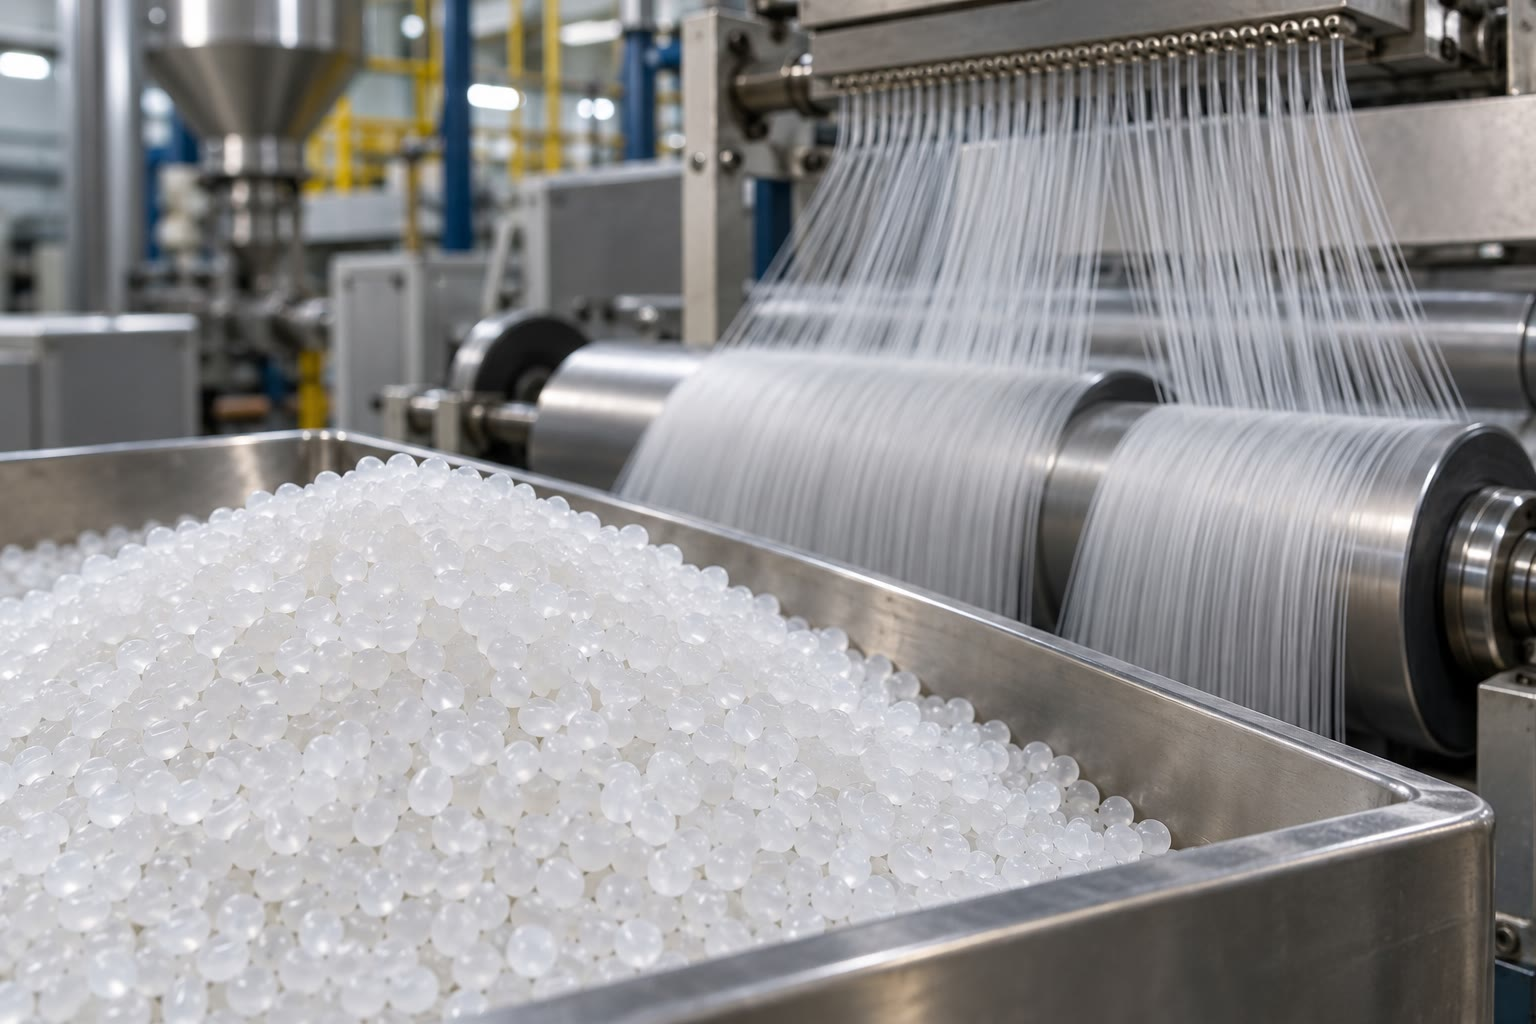
\includegraphics[width=0.58\linewidth]{images/book3/ai/b2-29-pellets.jpg}

{\small 工厂中的聚合物颗粒，即热塑性塑料的销售形态；纤维正从喷丝头
被拉出并卷到其后方的旋转辊上（示意图）。}
\end{omfigure}

\begin{history}[收率达到 99~\% 仍不够]
\begin{minipage}[t]{0.2\linewidth}
\vspace{0pt}
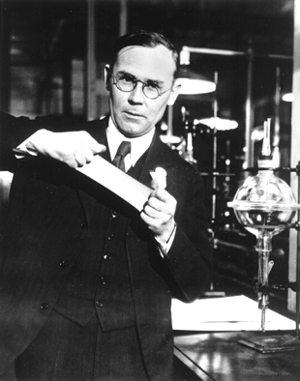
\includegraphics[width=\linewidth]{images/book3/carothers.jpg}
\end{minipage}\hfill
\begin{minipage}[t]{0.76\linewidth}
\vspace{0pt}
华莱士·卡罗瑟斯是一位年轻的大学讲师，被招募到工业实验室从事
基础研究，他用人们熟知的反应构建长分子，其结果有力地支持了
当时仍有争议的观点：聚合物只是普通分子，不过是非常长的分子。他的团队
先制得聚酯，随后自1934年起制得聚酰胺；以他名字命名的方程解释了为何只有
极高的转化率才能得到纤维。尼龙于1939年投入生产。（照片：作者不详，
公有领域；维基共享资源。）
% ledger: hist:polyamides-1934, hist:nylon-production-1939
\end{minipage}
\end{history}

\begin{safety}{\ghs[5mm]{GHS01}\,\ghs[5mm]{GHS02}\,\ghs[5mm]{GHS05}\,\ghs[5mm]{GHS07}\,\ghs[5mm]{GHS08}\,\ghs[5mm]{GHS09}}
苯乙烯易燃，且有健康危害。过氧化二苯甲酰干燥时为爆炸性氧化剂，
应保持潮湿并冷藏。1,6-己二胺和己二酸对眼睛有腐蚀性。
% ledger: ghs:styrene, ghs:BPO, ghs:hexanediamine, ghs:adipic-acid
\end{safety}

\section{练习}

\begin{exercise}[$\star$]\label{exo:b2:polymer-synthesis:1}
写出聚乙烯、聚丙烯、聚氯乙烯、聚苯乙烯和尼龙-6,6 的重复单元。
\end{exercise}

\begin{exercise}[$\star$]\label{exo:b2:polymer-synthesis:2}
判断下列聚合物属于逐步聚合还是链式聚合：由乙二醇与对苯二甲酸制得的 PET；聚苯乙烯；
尼龙-6,6；聚甲基丙烯酸甲酯；由 2-羟基丙酸制得的聚乳酸？
\end{exercise}

\begin{exercise}[$\star$]\label{exo:b2:polymer-synthesis:3}
某聚苯乙烯的 $\bar X_n = 1000$。忽略端基，求 $\bar M_n$。
\end{exercise}

\begin{exercise}[$\star$]\label{exo:b2:polymer-synthesis:4}
一条聚丙烯分子链画成平面锯齿形，其甲基依次位于纸面前方，
后方、前方、后方……依此类推。指出其立构规整性类型。它能否结晶？
\end{exercise}

\begin{exercise}[$\star\star$]\label{exo:b2:polymer-synthesis:5}
某样品是两个组分等质量的混合物，其摩尔质量分别为 \qty{10}{kg/mol} 和
\qty{100}{kg/mol}。求 $\bar M_n$、$\bar M_w$ 及分散度。
\end{exercise}

\begin{exercise}[$\star\star$]\label{exo:b2:polymer-synthesis:6}
求配平的逐步聚合反应的 $\bar X_n$，取 $p = 0.98$ 与 $p = 0.995$。
\end{exercise}

\begin{exercise}[$\star\star$]\label{exo:b2:polymer-synthesis:7}
将二元酸与二元胺混合，二元胺按摩尔计过量 1~\%。能达到的最大
$\bar X_n$ 是多少？
\end{exercise}

\begin{exercise}[$\star\star$]\label{exo:b2:polymer-synthesis:8}
在自由基聚合中，引发剂浓度增为原来的两倍。聚合速率与
动力学链长各变为原来的多少倍？
\end{exercise}

\begin{exercise}[$\star\star$]\label{exo:b2:polymer-synthesis:9}
聚氯乙烯较为刚硬；由它制成的花园水管却很柔软，因为其中含有增塑剂，
即混入链间的小分子。请利用玻璃化转变加以解释。
\end{exercise}

\begin{exercise}[$\star\star\star$]\label{exo:b2:polymer-synthesis:10}
证明：将弗洛里质量分布 $w_x = x(1-p)^2p^{\,x-1}$ 视为连续变量 $x$ 的函数时，
在 $x = -1/\ln p$ 处取最大值，且该值接近 $\bar X_n$，前提是 $p$ 接近 1。
\end{exercise}

\begin{exercise}[$\star\star\star$]\label{exo:b2:polymer-synthesis:11}
PET 分两步制备：先将对苯二甲酸二甲酯与过量乙二醇反应，
得到对苯二甲酸双（2-羟乙基）酯并放出甲醇；再将该双酯在真空中加热，
使其聚合并放出乙二醇。写出两步反应式，并说明第二步如何
解决卡罗瑟斯方程所涉及的化学计量问题。
\end{exercise}

\begin{exercise}[$\star\star\star$]\label{exo:b2:polymer-synthesis:12}
单体 1 与单体 2 进行自由基共聚，共聚物的瞬时组成由下式给出：
$\dfrac{\mathrm d[\mathrm M_1]}{\mathrm d[\mathrm M_2]} = \dfrac{[\mathrm M_1](r_1[\mathrm M_1]
+ [\mathrm M_2])}{[\mathrm M_2]([\mathrm M_1] + r_2[\mathrm M_2])}$，其中 $r_1$ 与 $r_2$ 为
竞聚率（练习数据：$r_1 = 2.0$，$r_2 = 0.5$）。求由等摩尔投料所得
共聚物中两种链节的比值。若 $r_1 = r_2 = 0$，会发生什么？
\end{exercise}

\section{周末问题：千克级尼龙-6,6}

\begin{problem}[{周末问题——单体与尼龙盐、卡罗瑟斯方程、
刻意的配比失衡、弗洛里分布与释放的水}]
\label{pb:b2:polymer-synthesis:1}
尼龙-6,6 由 1,6-己二胺与己二酸制得。全程忽略端基。
摩尔质量（\unit{g/mol}）：C 12.011，H 1.008，N 14.007，O 15.999。
% ledger: aw:C, aw:H, aw:N, aw:O, ghs:hexanediamine, ghs:adipic-acid

\medskip
\noindent\textbf{第一部分——单体与重复单元。}
\begin{enumerate}
  \item 写出两种单体的化学式。
  \item 写出生成一个酰胺键的方程式。
  \item 两种单体先以 1\,:\,1 的比例结合成盐，并从溶液中结晶析出。为什么？
  \item 给出尼龙-6,6 的重复单元、其化学式及其摩尔质量。
  \item 链中由单体衍生的单元的平均摩尔质量 $M_0$ 是多少？
  \item 名称中“6,6”的两个数字分别计数什么？
\end{enumerate}

\medskip
\noindent\textbf{第二部分——卡罗瑟斯方程。}
\begin{enumerate}[resume]
  \item 计算 $\bar X_n$ 与 $\bar M_n$，取 $p = 0.98$。
  \item 同样取 $p = 0.99$ 计算。
  \item 解释评注“产率 99~\% 仍不够”。
  \item 反应进度为多少时 $\bar M_n = \qty{10}{kg/mol}$？
  \item 实际中如何将反应进度推到如此之高？
  \item 为什么单体必须非常纯？
\end{enumerate}

\medskip
\noindent\textbf{第三部分——刻意的配比失衡。}
\begin{enumerate}[resume]
  \item 二胺以 1~\% 的摩尔过量使用。计算 $r$。
  \item 计算此时能达到的最大 $\bar X_n$ 与 $\bar M_n$。
  \item 在此配比失衡下计算 $\bar X_n$，取 $p = 0.99$。
  \item 反应结束时，哪些基团封住了链端？
  \item 有时会加入少量乙酸。它对链有何作用？
  \item 生产商为何要有意限制链长？
\end{enumerate}

\medskip
\noindent\textbf{第四部分——分布与质量平衡。}
\begin{enumerate}[resume]
  \item 对于等配比混合物，在 $p = 0.99$ 时给出分散度。
  \item 计算 $\bar M_w$，取 $p = 0.99$。
  \item 在 $p = 0.99$ 时，仍未反应的单体
        占分子数的比例与占质量的比例各为多少？
  \item 质量分布在哪一链长附近达到最大？
  \item 计算每千克尼龙-6,6 所释放的水的质量。
  \item 熔融纺丝为何要求 $\bar M_n$ 位于某一范围内？
  \item 对于等配比混合物，给出使 $\bar M_n = \qty{20}{kg/mol}$ 的反应进度。
\end{enumerate}
\end{problem}
